\documentclass[tikz,border=2pt,11pt]{standalone}
\usetikzlibrary{positioning}
\usetikzlibrary{arrows.meta}
\usetikzlibrary{patterns}
\usetikzlibrary{calc}
\usetikzlibrary{decorations.pathreplacing}
\usepackage{amsmath}
\usepackage{amssymb}
\usepackage{graphicx}
\usepackage{xcolor}
\usepackage{tikz}
\newcommand{\R}{\mathbb R}
\newcommand{\N}{\mathbb N}
\newcommand{\Z}{\mathbb Z}
\newcommand{\eps}{\varepsilon}
\newcommand{\Id}{\operatorname{id}}
\newcommand{\id}{\operatorname{id}}
\newcommand{\cH}{\mathcal H}
\newcommand{\cL}{\mathcal L}
\newcommand{\norm}[1]{\left\lVert #1\right\rVert}
\newcommand{\abs}[1]{\left\lvert #1\right\rvert}
\newcommand{\ind}{\mathbf 1}
\newcommand{\op}{\mathrm{op}}
\DeclareMathOperator{\Lip}{Lip}
\DeclareMathOperator{\supp}{supp}
\DeclareMathOperator{\diam}{diam}
\DeclareMathOperator{\dist}{dist}
\DeclareMathOperator{\rank}{rank}
\DeclareMathOperator{\GL}{GL}
\DeclareMathOperator{\tr}{tr}
\DeclareMathOperator{\conv}{conv}
\DeclareMathOperator{\relint}{relint}
\DeclareMathOperator{\interior}{int}
\DeclareMathOperator{\osc}{osc}
\DeclareMathOperator{\sgn}{sgn}
\begin{document}
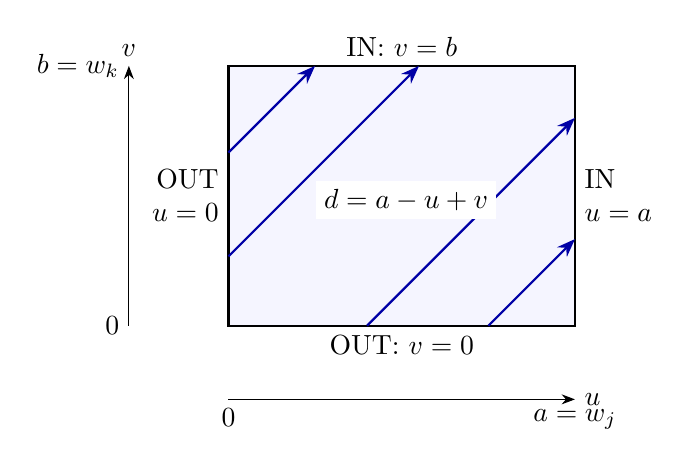
\begin{tikzpicture}[x=1.1cm,y=1.1cm,>=Stealth]
 \fill[blue!4] (0,0) rectangle (4,3);
 \draw[thick] (0,0) rectangle (4,3);
 \draw[blue!65!black,thick,->] (3,0)--(4,1);
 \draw[blue!65!black,thick,->] (1.6,0)--(4,2.4);
 \draw[blue!65!black,thick,->] (0,.8)--(2.2,3);
 \draw[blue!65!black,thick,->] (0,2)--(1,3);
 \node[below] at (2,0) {OUT: $v=0$};
 \node[left,align=right] at (0,1.5) {OUT\\$u=0$};
 \node[above] at (2,3) {IN: $v=b$};
 \node[right,align=left] at (4,1.5) {IN\\$u=a$};
 \draw[->] (0,-.85)--(4,-.85) node[right] {$u$};
 \node[below] at (0,-.85) {$0$};
 \node[below] at (4,-.85) {$a=w_j$};
 \draw[->] (-1.15,0)--(-1.15,3) node[above] {$v$};
 \node[left] at (-1.15,0) {$0$};
 \node[left] at (-1.15,3) {$b=w_k$};
 \node[fill=white,inner sep=3pt] at (2.05,1.45) {$d=a-u+v$};
\end{tikzpicture}
\end{document}
